\documentclass[12pt,a4paper]{paper}
\usepackage[utf8]{inputenc}
\usepackage[english]{babel}
\usepackage{amsmath}
\usepackage{enumitem}
\usepackage{amsfonts}
\usepackage{amssymb}
\usepackage[left=2cm,right=2cm,top=2cm,bottom=2cm]{geometry}
\usepackage{Sweave}
\begin{document}
\title{STAT646 - Homework 3\\\small{Daniel Osorio - dcosorioh@tamu.edu\\Department of Veterinary Integrative Biosciences\\Texas A\&M University}}
\maketitle
\Sconcordance{concordance:Osorio_Daniel_HW3.tex:Osorio_Daniel_HW3.Rnw:%
1 8 1 1 0 9 1 4 0 1 3 1 4 3 0 1 2 1 0 5 1 1 3 2 0 1 1 1 5 4 0 1 2 1 0 1 %
3 6 0 1 2 2 1}

\begin{enumerate}
\item Read the minfi tutorial: \\https://www.bioconductor.org/help/course-materials/2015/BioC2015/methylation450k.html
\item Read the Breacher analysis2.pdf. Take the RGset data, the phenotype data (uploaded at eCampus) and perform the following steps:
\begin{enumerate}
\item Normalize the data using SWAN normalization.
\begin{Schunk}
\begin{Sinput}
> #load("rgset_breacher.Rdata")
\end{Sinput}
\end{Schunk}
\item Recreate all the plots from the Breacher\_analysis2.pdf file.
\begin{Schunk}
\begin{Sinput}
> phenoData <- read.csv(file = "Phenotype_Breacher_HM450.csv", 
+                       row.names = 1, 
+                       stringsAsFactors = FALSE)
> excludeS <- c('879', '4667', '5505', '7725', '3F05_1_2', 
+               '3F05_10_2', 'Leuk_ZC', 'Leuk_FH', '3D03_10_2')
> phenoData <- phenoData[!rownames(phenoData) %in% excludeS,]
> bL <- phenoData[phenoData$sample == 1,]
> colnames(bL)[7] <- "Breaches"
> bL$Breaches[bL$Breaches == "1/9/2016"] <- "1-9"
> bL$Breaches[bL$Breaches %in% c("400+", "200-399")] <- "200+"
> bL$Breaches <- factor(x = bL$Breaches, 
+                       levels = c("0", "1-9", "10-39", 
+                                  "40-99", "100-199", "200+"))
> par(mar=c(3,3,2,1), mgp = c(1.5,0.5,0), mfrow = c(1,2))
> plot(x = bL$Breaches, 
+      main = "# Breaches", 
+      xlab = "Categories", 
+      ylab = "Breaches",
+      las = 1)
> pie(x = c('65.625%' = 70,'34.375%'=30), 
+     col = c("red", "skyblue"))
> legend("topright", 
+        legend = c("<39", ">39"), 
+        fill = c("red", "skyblue"), bty = "n")
\end{Sinput}
\end{Schunk}
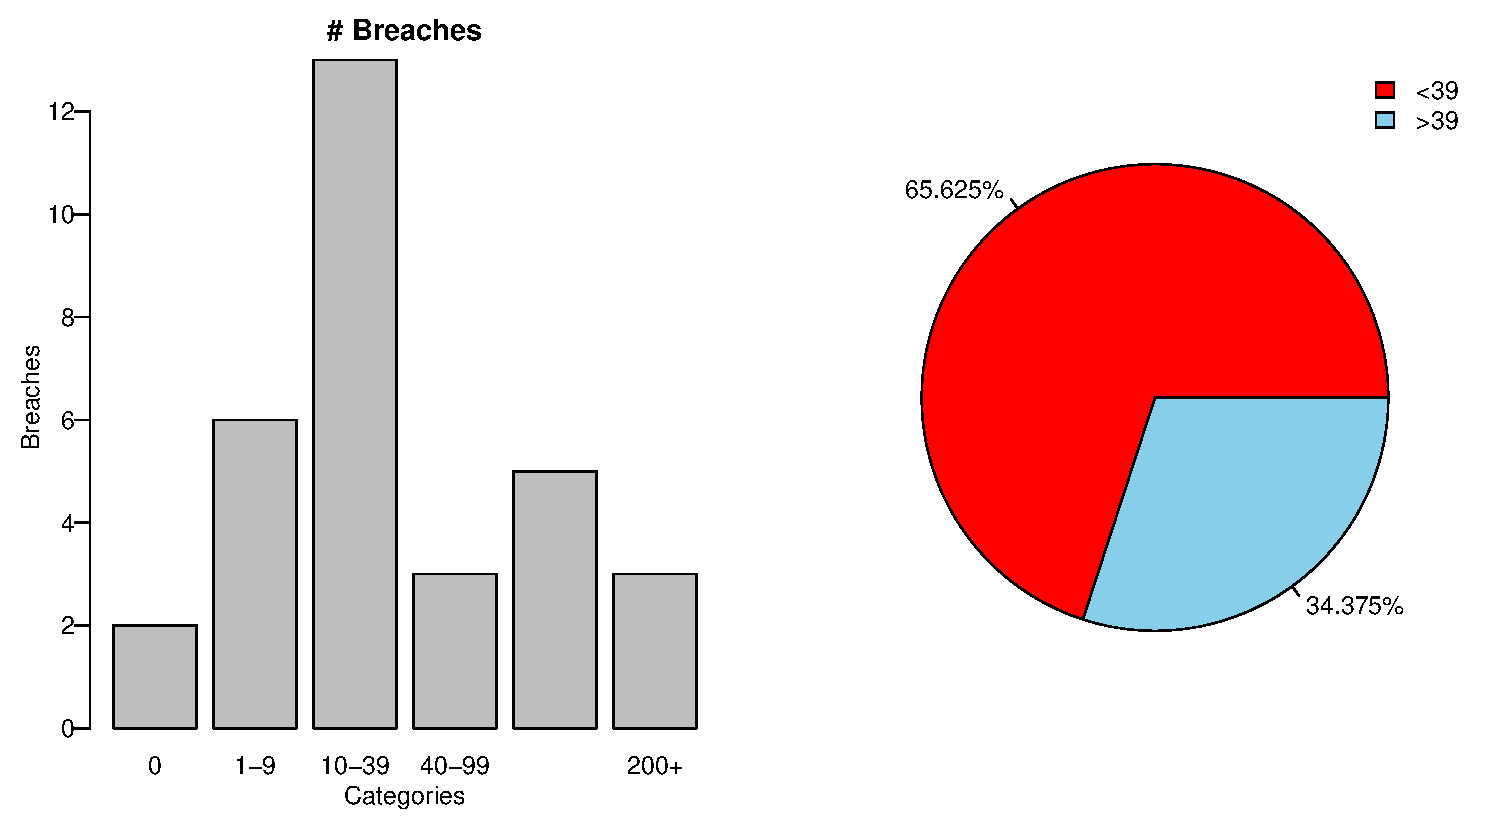
\includegraphics{Osorio_Daniel_HW3-002}
\end{enumerate}
\end{enumerate}
\end{document}
